% \vspace{-6mm}
\section{}
\vspace{-2mm}
    \subsection{CODE}
    \label{sec: 3code}
        \subsubsection{Network3.ned}
            \vspace{-2mm}
            \begin{listing}[h!]
            \inputminted[framerule = 1pt,framesep = 2mm , frame = lines, fontsize=\footnotesize]{c}{./code/week10/Experiment03/01_Network.cc}
            \vspace{-3mm}
            \caption{\footnotesize experiment 3, Network3.ned}
            \end{listing}
            \vspace{-6mm}    
\clearpage
        \subsubsection{AP.cc}
            \vspace{-2mm}
            \begin{listing}[h!]
            \inputminted[framerule = 1pt,framesep = 2mm , frame = lines, fontsize=\scriptsize]{c}{./code/week10/Experiment03/02_AP.cpp}
            \vspace{-3mm}
            \caption{\footnotesize experiment 3, AP.cc}
            \end{listing}
            \vspace{-6mm}    
        \subsubsection{client.cc}
            \vspace{-2mm}
            \begin{listing}[h!]
            \inputminted[framerule = 1pt,framesep = 2mm , frame = lines, fontsize=\scriptsize]{c}{./code/week10/Experiment03/03_client.cpp}
            \vspace{-3mm}
            \caption{\footnotesize experiment 3, client.cc}
            \end{listing}
            \vspace{-6mm}   
\clearpage 
        \subsubsection{router.cc}
            \vspace{-2mm}
            \begin{listing}[h!]
            \inputminted[framerule = 1pt,framesep = 2mm , frame = lines, fontsize=\footnotesize]{c}{./code/week10/Experiment03/04_router.cpp}
            \vspace{-3mm}
            \caption{\footnotesize experiment 3, router.cc}
            \end{listing}
            \vspace{-6mm}    
        \subsubsection{server.cc}
            \vspace{-2mm}
            \begin{listing}[h!]
            \inputminted[framerule = 1pt,framesep = 2mm , frame = lines, fontsize=\footnotesize]{c}{./code/week10/Experiment03/05_server.cpp}
            \vspace{-3mm}
            \caption{\footnotesize experiment 3, server.cc}
            \end{listing}
            \vspace{-6mm}    

    \subsection{SIMULATION RESULTS}
    \vspace{-1mm}
    client/ server/ Access Pint(AP) 2개/ router의 4개로 구성된 네트워크를 구성한다. 
    client/ server와 AP 간의 연결은 무선으로, AP와 router 간의 연결은 유선으로 구성한다. 
    
    Simulation이 시작되면 client → AP2 → router → AP1 → server 순서로 메세지를 전송한다.
    메세지를 server가 수신하면 server → AP1 → router → AP2 → client 순서로 메세지를 재전송한다.
    \vspace{-3mm}
        \subsubsection{SCREENSHOT}
        시뮬레이션의 결과에서 구성한 모듈 사이에서 메세지의 전송과 재전송을 잘 담기 위해서 화면녹화 screenshot 영상을 촬영해 youtube에 업로드하였다. 해당 영상은 아래의 링크를 클릭해 이동이 가능하다.
        \vspace{-10mm}
            \begin{center}
                \item \href{https://youtu.be/D_AXEdjixsc}
            	{Youtube link of Week10 Experiment 03 Simulation Results Screenshot Video}
            \end{center}
        \vspace{-6mm}
\clearpage
        % 사진 1 2개는 넣어 주자
            \begin{figure}[h!]
            \centering
            \subfloat[Simulation Screenshot 2]{
                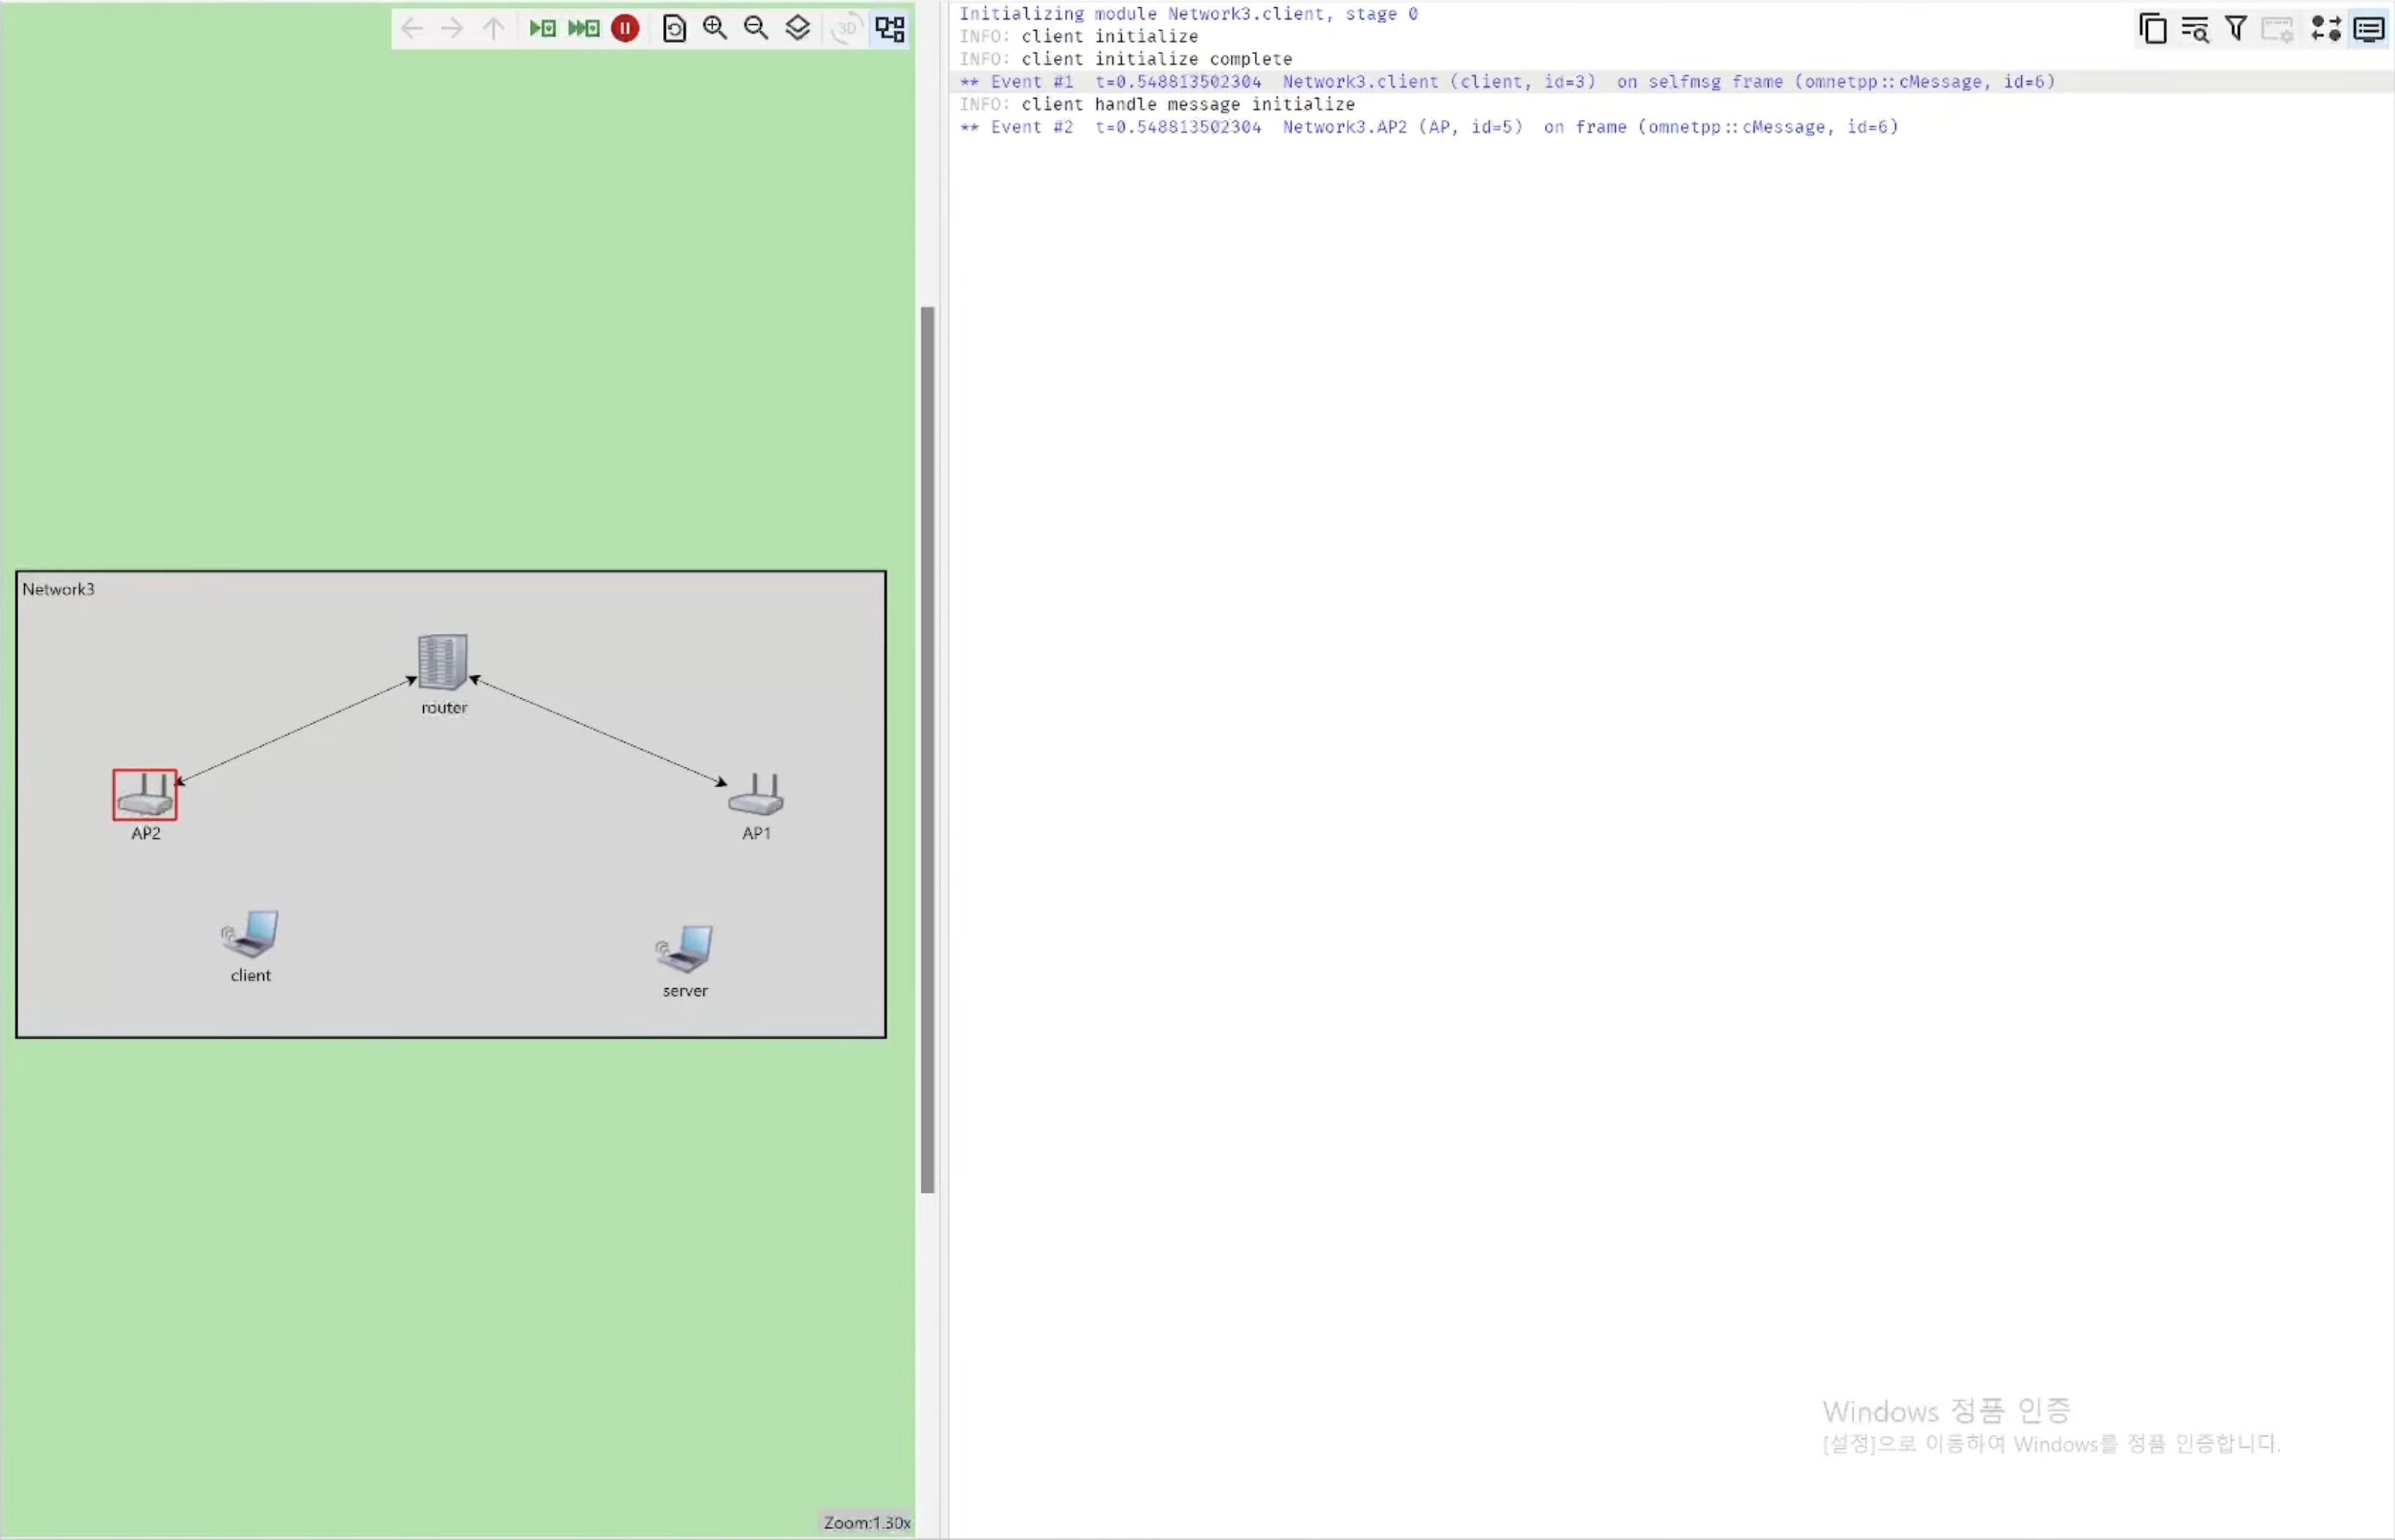
\includegraphics[width=0.47\textwidth]{image/week10/3-1-1.png}
            }\hspace{3mm}
            \subfloat[Simulation Screenshot 2]{
                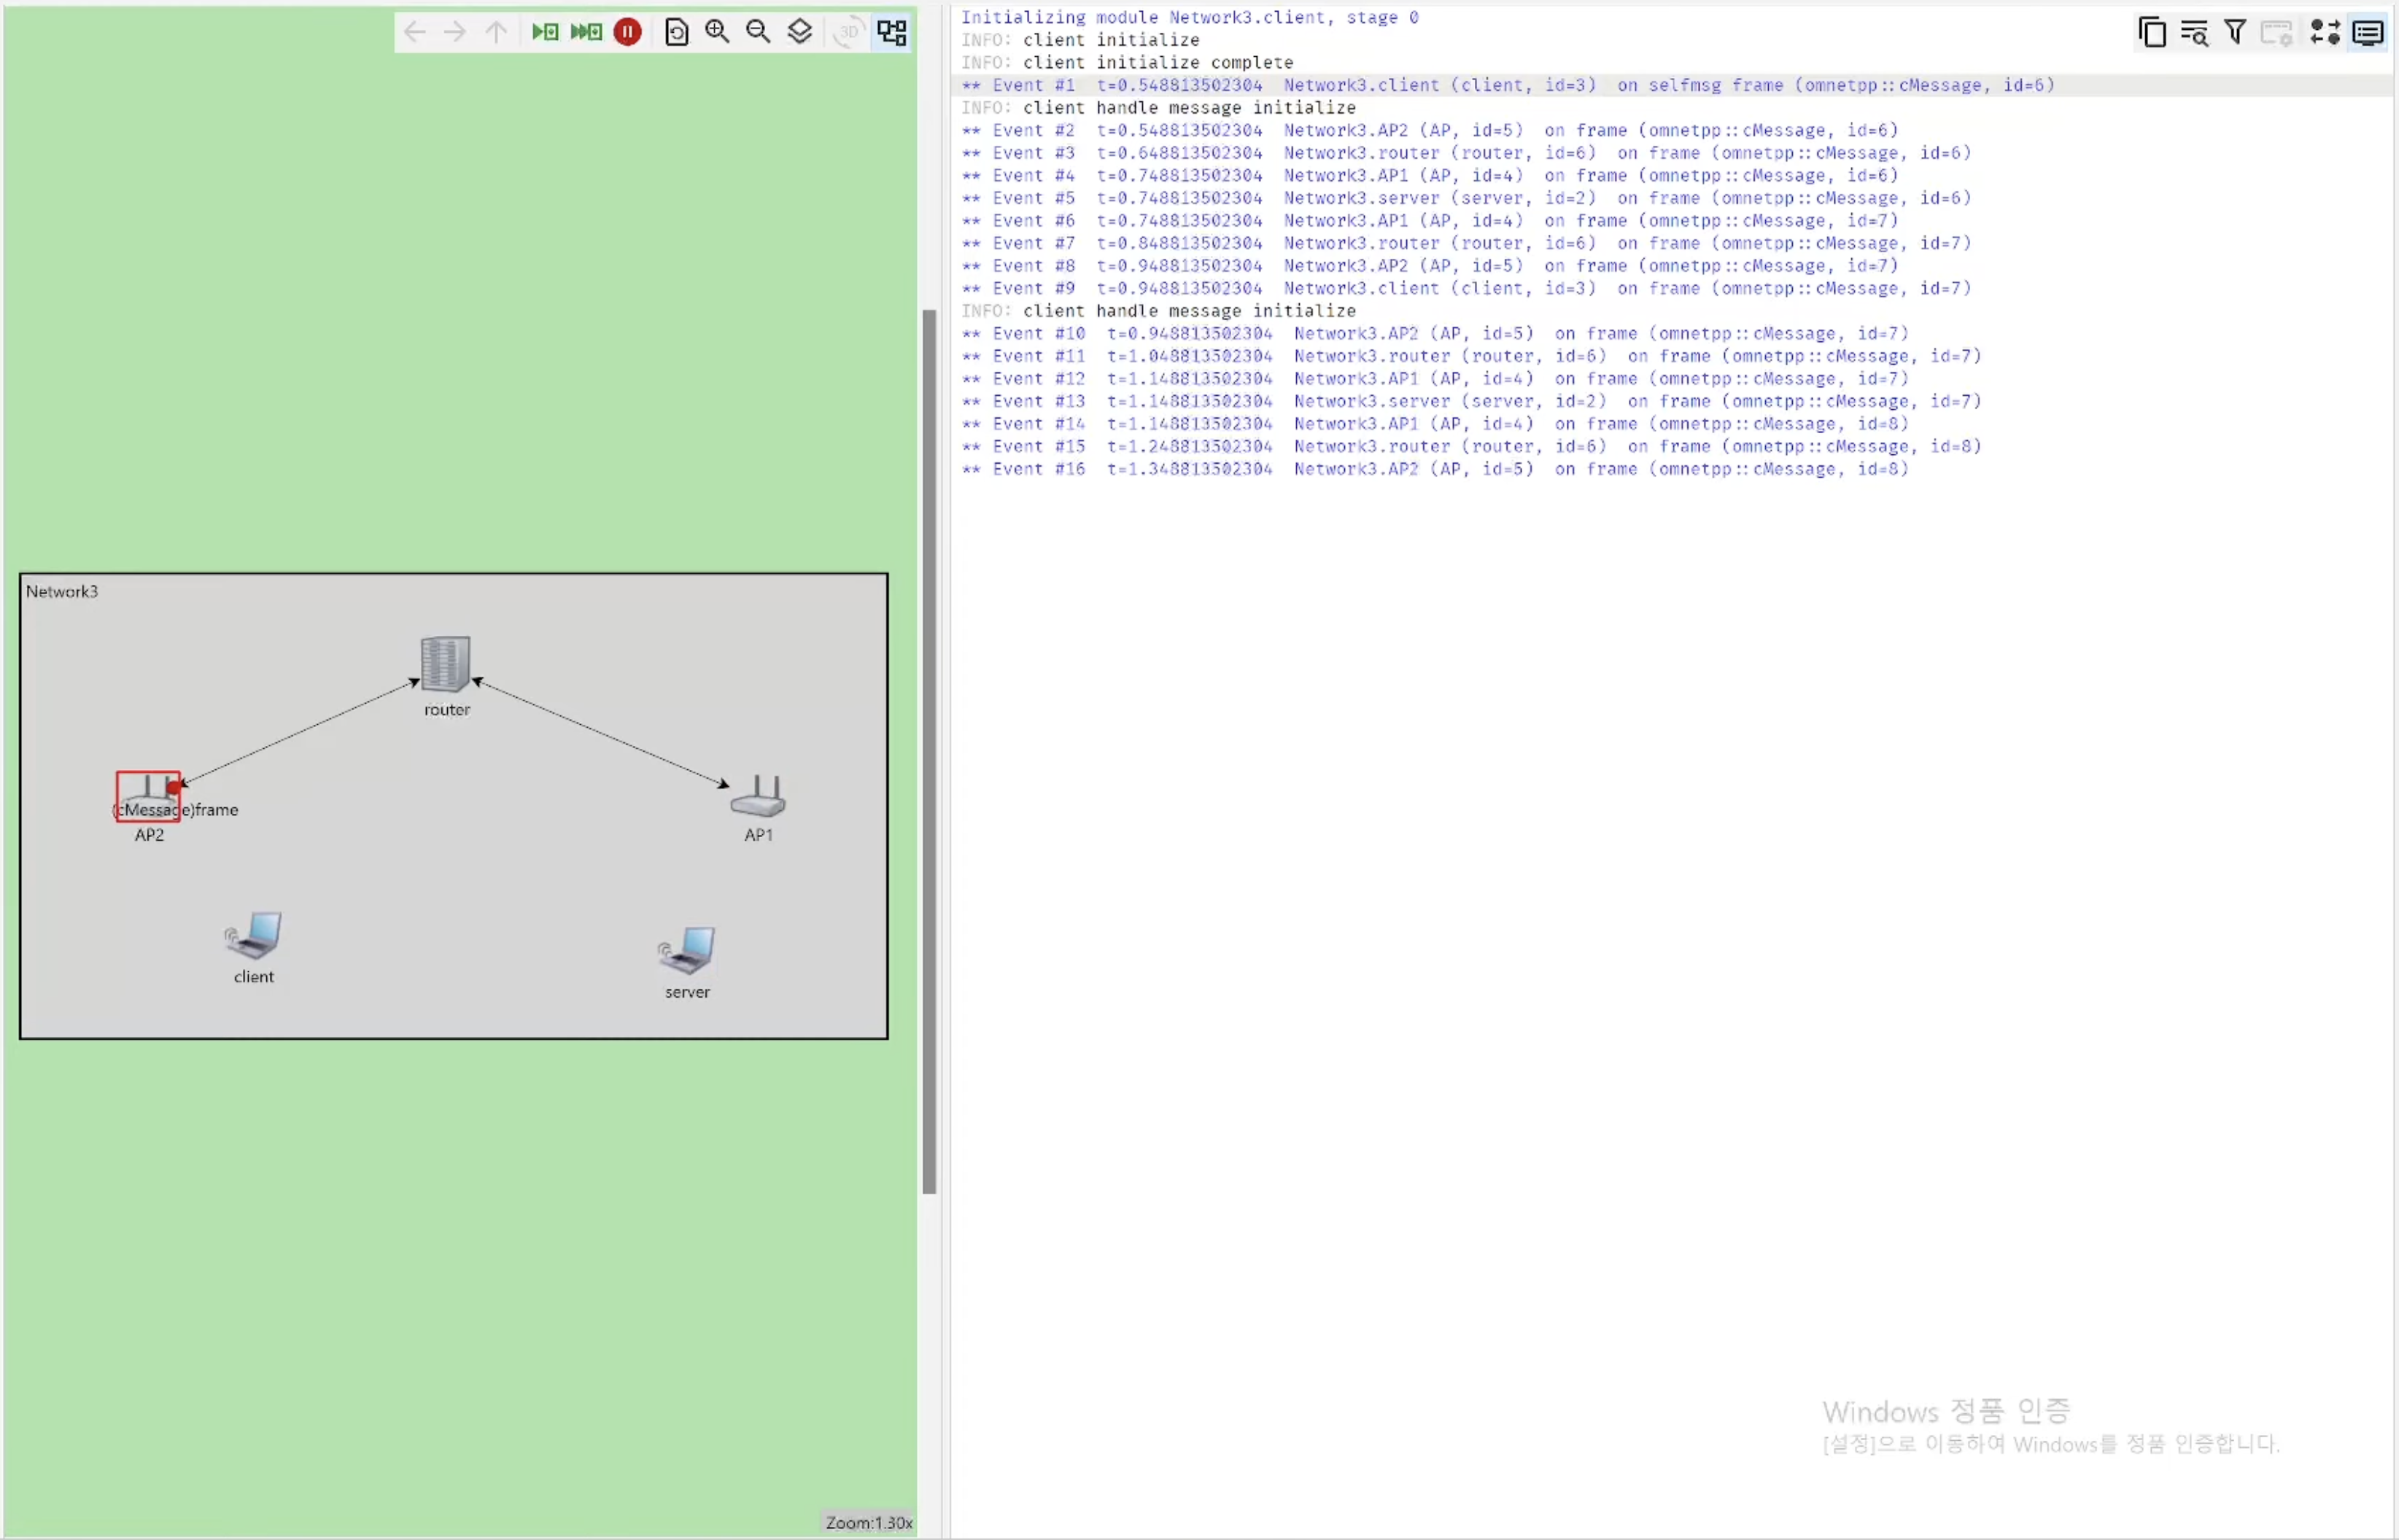
\includegraphics[width=0.47\textwidth]{image/week10/3-1-2.png}
            }
            \caption{Experiment 03 Simulation Results Screenshot}
            \end{figure}
            \vspace{-6mm}
        \subsubsection{RESULTS GRAPH}
            \vspace{-4mm}
            \begin{figure}[!h]\centering 
            	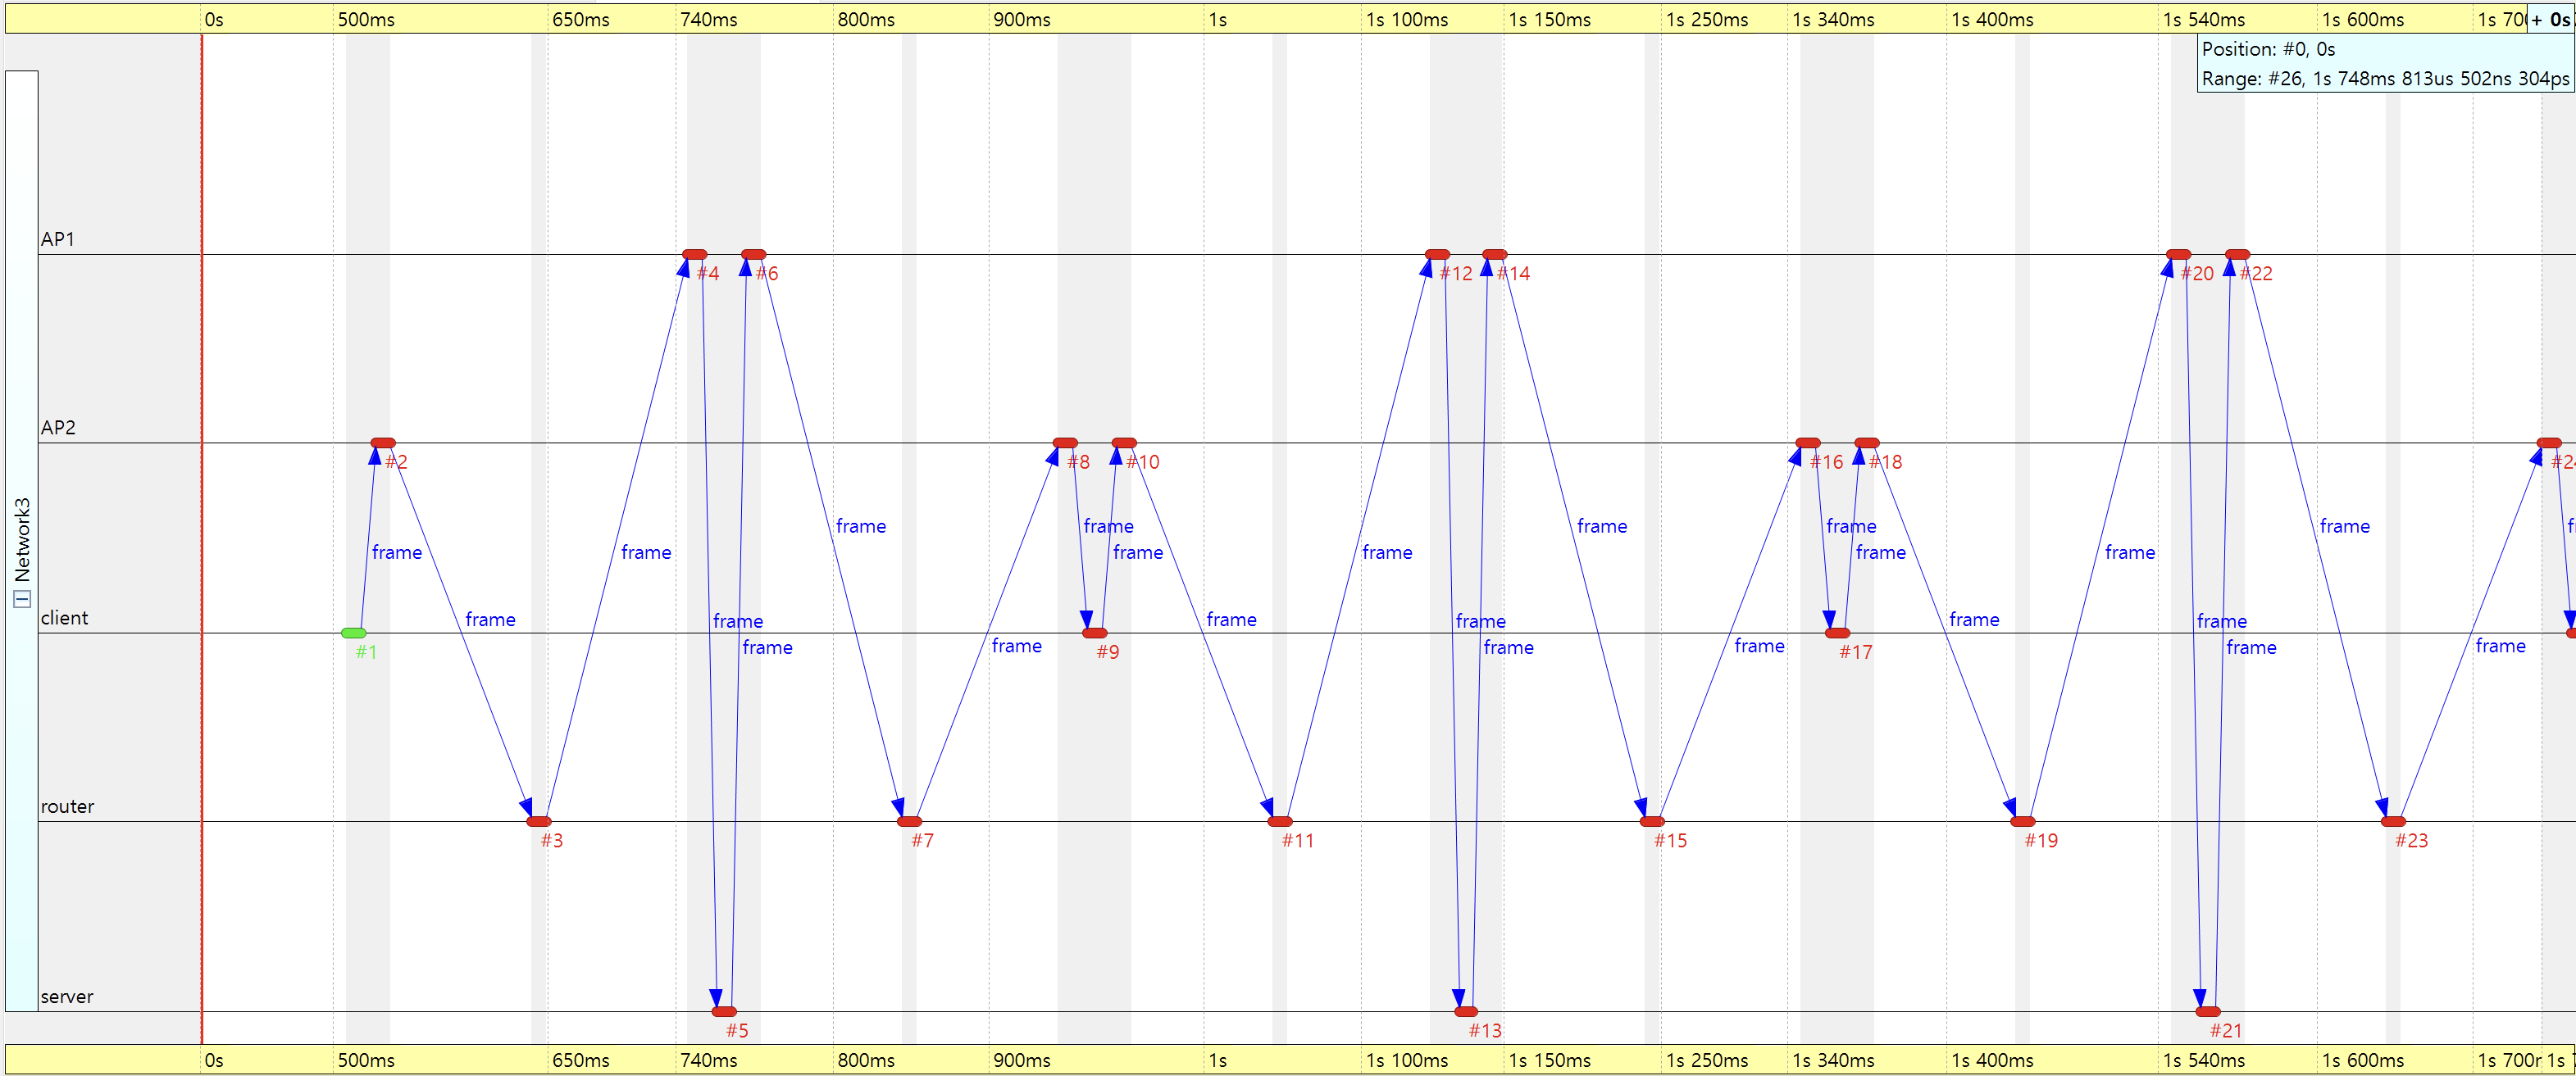
\includegraphics[width=.99\textwidth]{image/week10/3-2.png}
            	\caption{\footnotesize
            	Experiment 03 Simulation Results Sequence Chart}
            	\vspace{-10pt}
            \end{figure}
            \vspace{-4mm}
        \subsubsection{DISCUSSION}
        \ref{sec: 3code} code에서 설명한 과정에서 graph에서도 확인할 수 있듯이, 실험조건에 connection의 msg 전달 경로에 대한 부만 언급이되고 유선 무선환경에 따른 delay설정에 관한 부분이 없어 무선환경을 가정하는 server/ client 와 AP 간의 연결에는 Experiment 1 과 같은 random 시간에 msg를 보내는 부분을 제외하고 바로 msg를 보내는 동작을하게 하였고, 유선환경을 가정하는 AP와 router간의 유선연결에서는 100ms의 delay를 Experiment2와 동일하게 설정해 주었다. 
        
        Graph는 총 3cycle 동안의 msg 이동을 기록했으며, 각 module간의 msg 전송간의 delay또한 앞서 설명한 부분과 같이 동작함을 확인할 수 있었다. 